GSM (Global System for Mobile Communications) è uno standard della seconda generazione (2G) per le comunicazioni mobili.
È stato impiegato per la prima volta nel 1991 in Finlandia, venendo standardizzato dall'ETSI (European Telecommunications Standards Institute)
e successivamente adottato in tutto il mondo.
La prima architettura GSM era a commutazione di circuito, per essere completamente integrata con le reti telefoniche fisse.
\section{Architettura}
\begin{figure}[H]
	\centering
	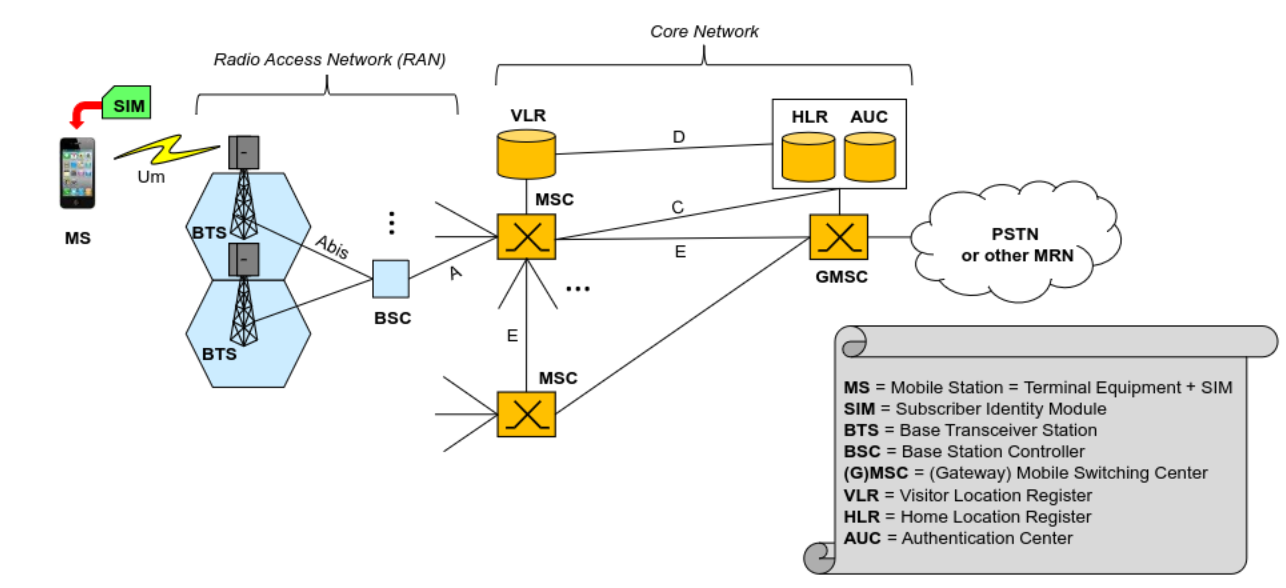
\includegraphics[width=\textwidth]{pictures/9/architecture.png}
	\caption{Architettura di rete GSM}
\end{figure}
Cominciamo elencando i componenti principali dell'architettura GSM:
\begin{itemize}
	\item \textbf{Mobile Station (MS)}: dispositivo mobile che include un terminal equipment (TE) e un subscriber identity module (SIM).
	\item \textbf{Base transceiver station (BTS)}: base station nelle reti GSM, gestisce le connessioni al livello fisico con gli MS ed esegue i comandi di allocazioni delle risorse ricevuti dal BSC.
	\item \textbf{Base Station Controller (BSC)}: controlla tutte le risorse radio dei BTS ad esso collegate. Tutte le BTS collegate a un BSC appartengono alla stessa Location Area.
	\item \textbf{Mobile Switching Center (MSC)}: componente responsabile dell'instradamento delle chiamate, incluse funzioni di controllo/signaling per gestire le chiamate e la mobilità. Simile al phone exchange in PSTN.
	\item \textbf{Visitor Location Register (VLR)}: database associato a un MSC, memorizza le informazioni temporanee su gli utenti che visitano le celle coperte dai BTS controllati dai BSC che sono collegati al MSC.
	\item \textbf{Gateway MSC (GMSC)}: MSC connesso alla PSTN o altre reti radiomobili, implementa funzioni di signaling inter-rete.
	\item \textbf{Home Location Register {HLR}}: database centrale che memorizza le informazioni permanenti su ogni utente, e le informazioni dinamiche sulla posizione (e.g. VLR visitate).
	\item \textbf{Authentication Center (AUC)}: autentica le SIM che cercano di accedere alla core network. 
\end{itemize}
\section{Layer fisico}
IN GSM, vengono utilizzate sia FDM che TDM.
Lo spettro viene diviso in porzioni (\textbf{carrier}) e su ognuna di queste viene effettuato TDM per dividere in diversi \textbf{timeslots}.
Questi timeslots vengono usati per mandare dati appartenenti a diversi canali (voce/traffico e controllo).
L'upstream e il downstream sono in frequenze diverse (Frequency division duplexing).
\begin{figure}[H]
	\centering
	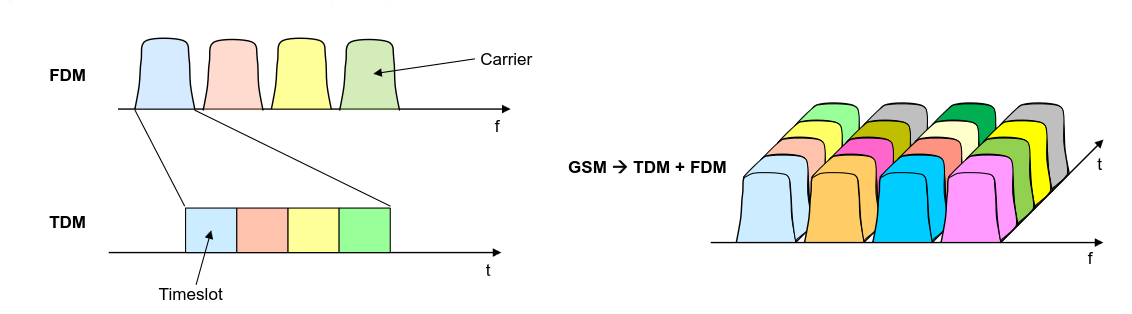
\includegraphics[width=\textwidth]{pictures/9/layerFisico.png}
	\caption{Frequenze utilizzate in GSM}
\end{figure}
\section{Canali di traffico e controllo}
I \textbf{canali di traffico (TCH)} vengono usati per trasportare i dati vocali.
Diversi \textbf{canali di controllo} vengono usati per trasportare il signaling, tra cui:
\begin{itemize}
	\item \textbf{BCCH (Broadcast Control Channel)}: porta informazioni generali sui BTS, tra cui il BTS ID, il Mobile Network Code (MNC) e la Location Area Identity (LAI) sul canale di downlink.
	Viene sempre trasmesso a potenza massima, e viene usato come canale di beacon.
	\item \textbf{PCH (Paging Channel)}: usato dal BTS per trasmettere i messaggi di paging quando un MS ha una chiamata in arrivo (downlink).
	Mandato in broadcast da tutti i BTS nella Location Area.
	Viene inoltre usato per mandare gli SMS.
	\item \textbf{RACH (Random Access Channel)}: usato dagli MS per accedere alla rete (chiamate in uscita, location update etc.), viene mandato in uplink. Basato su architettura slotted-Aloha.
	\item \textbf{AGCH (Access Grant Channel)}: usato per le risposte alle richieste provenienti dal RACH (downlink). Contiene informazioni sul SDCCH da usare.
	\item \textbf{SDCCH (Stand-alone Dedicated Control Channel)}: assegnato durante lo scambio di messaggi RACH/AGCH per ulteriori procedure di breve durata.
	\item \textbf{SACCH (Slow Associated Control Channel)}: usato per scambiare misurazioni durante la connessione tra MS e BTS, ad esempio potenza del segnale.
	\item \textbf{FACCH (Fast Addociated Control Channel)}: trasporta il signaling generato durante l'handover e setup delle chiamate.
\end{itemize}
\begin{figure}[H]
	\centering
	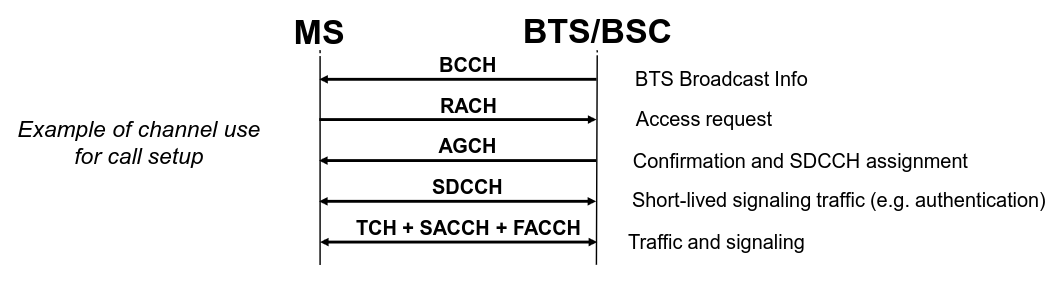
\includegraphics[width=\textwidth]{pictures/9/controlChannels.png}
	\caption{Canali di controllo in GSM}
\end{figure}
\section{Identificatori GSM}
Gli identificatori GSM sono usati per identificare in modo univoco i dispositivi, le reti e le aree geografiche.
\begin{itemize}
	\item \textbf{MSISDN (Mobile Station ISDN Number)}: numero E.164, usato da reti esterne per raggiungere le MS (permanente e pubblico).
	\item \textbf{MSRN (Mobile Station Roaming Number)}: numero E.164, usato per instradare la chiamata nella rete mobile fino al raggiungimento del MSC (temporaneo e privato).
	\item \textbf{IMSI (International Mobile Subscriber Identifier)}: identificatore univoco di una MS, permanentemente scritto nella SIM, memorizzato nel HLR.
	\item \textbf{TMSI (Temporary Mobile Station Identifier)}: identificatore temporaneo di una MS allocato dal VLR e memorizzato in esso e nella SIM.
	\item \textbf{LAI (Location Area Identity)}: Una location area in GSM è un insieme di BTS gestiste dallo stesso BSC. Hanno un identificatore univoco, viene memorizzato nella SIM e nel VLR per ogni MS.
\end{itemize}
\section{Sicurezza}
Per ragioni di sicurezza, il VLR assegnato al momento alloca per la MS un TMSI, e la associazione TMSI-IMSI viene memorizzata nello stesso VLR.
Per ogni location update che riguarda diversi MSC un nuovo TMSI viene allocato alla MS.
Quando una MS vuole accedere a una rete, trasmette il suo TMSI e inizia il processo di autenticazione.
Se il TMSI non è disponibile, l'IMSI viene trasmesso in chiaro, e questo è un punto debole del sistema.
\subsection{Autenticazione e cifratura}
Le operazioni di sicurezza (autenticazione e cifratura) sono gestite dalla SIM/TE (ovvero la MS) e dal BTS/MSC/AUC (ovvero la rete).
I parametri sono:
\begin{itemize}
	\item $K_i$: la chiave univoca da 128 bit memorizzata sia nell'AUC e nella SIM.
	\item RAND: numero casuale da 128 bit generato dall'AUC e inviato alla MS attraverso l'MSC. 
\end{itemize}
Gli algoritmi utilizzati sono:
\begin{itemize}
	\item \textbf{A3}: algoritmo di autenticazione, contenuto sia nell'AUC che nella SIM.
	\item \textbf{A8}: algoritmo per la generazione della chiave di cifratura $K_c$, contenuto sia nell'AUC che nella SIM.
	\item \textbf{A5}: algoritmo di cifratura del flusso, contenuto sia nella MS (\underbar{non} nella SIM) e nel BTS.
\end{itemize}
\begin{figure}[H]
	\centering
	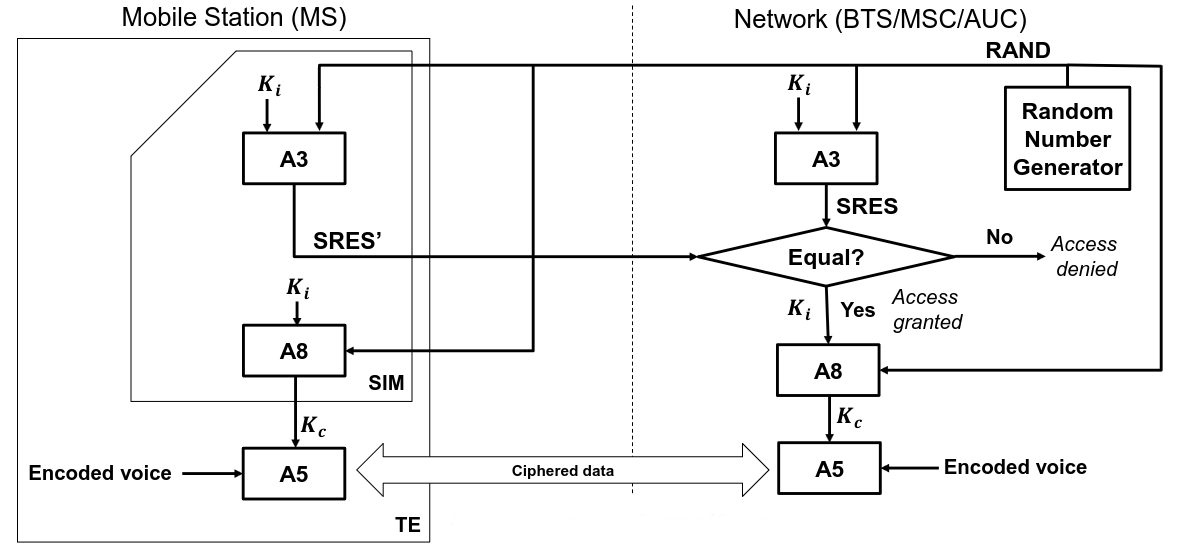
\includegraphics[width=\textwidth]{pictures/9/authentication.png}
	\caption{Autenticazione e cifratura in GSM}
\end{figure}
\begin{figure}[H]
	\centering
	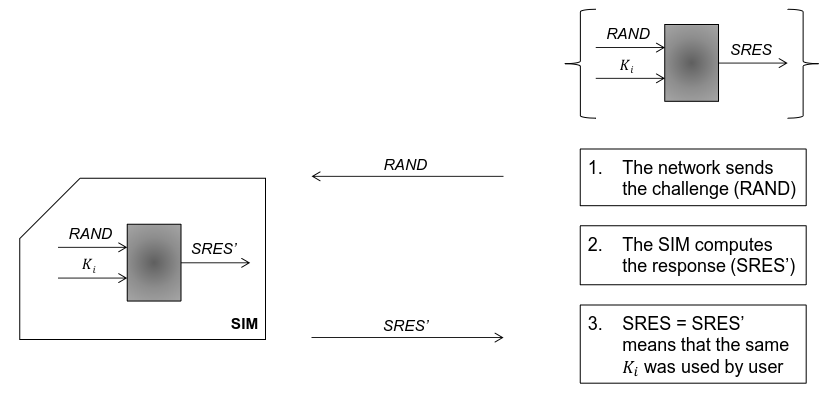
\includegraphics[width=0.7\textwidth]{pictures/9/recapCipher.png}
	\caption{Recap dei processi di autenticazione e cifratura in GSM}
\end{figure}
N.B. :
\begin{itemize}
	\item L'autenticazione GSM garantisce la legittimità della SIM, l'identità dell'utente viene verificata dalla sua abilità di attivare la SIM (ovvero di conoscere il PIN).
	\item L'autenticazione sulla rete non è verificata! Si possono effettuare attacchi man-in-the-middle attraverso i catcher di IMSI.
\end{itemize}
\section{Accensione di una MS}
Quando una MS viene accesa, esegue le seguenti operazioni:
\begin{enumerate}
	\item \textbf{Cell selection}: la MS seleziona la BTS a cui connettersi, scegliendo quella con la potenza del segnale più alta (emessa dal BCCH).
	\item \textbf{Registrazione}: la MS informa il MSC che è attivo, ci sono due tipi di scenari:
	\begin{itemize}
		\item \textbf{IMSI Attach}: Il LAI ricevuto dalla rete è uguale a quello memorizzato nella SIM, nel caso il telefono venga spento e riacceso nella stessa location area. L'IMSI viene marcato come attivo nel VLR.
		\item \textbf{Location Update}: Il LAI ricevuto dalla rete è diverso da quello memorizzato nella SIM. Viene inizializzato il processo di location update.
	\end{itemize}
\end{enumerate}
\section{Location update}
Una location update può avvenire in due modi:
\begin{itemize}
	\item Le due LA sono servite dallo stesso MSC/VLR
	\begin{figure}[H]
		\centering
		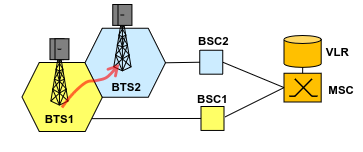
\includegraphics[width=0.5\textwidth]{pictures/9/sameMSC.png}
		\caption{Location update tra due LA servite dallo stesso MSC/VLR}
	\end{figure}
	\begin{figure}[H]
		\centering
		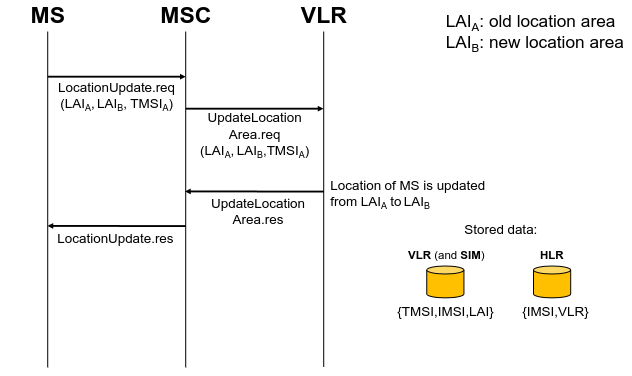
\includegraphics[width=0.8\textwidth]{pictures/9/sameMSCsequence.png}
		\caption{Diagramma di sequenza per location update tra due LA servite dallo stesso MSC/VLR}
	\end{figure}
	\item Le due LA sono servite da MSC/VLR diversi
	\begin{figure}[H]
		\centering
		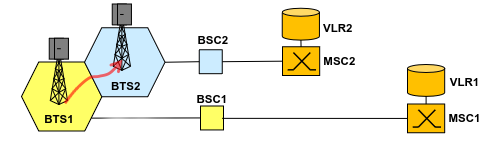
\includegraphics[width=0.6\textwidth]{pictures/9/differentMSC.png}
		\caption{Location update tra due LA servite da MSC/VLR diversi}
	\end{figure}
	\begin{figure}[H]
		\centering
		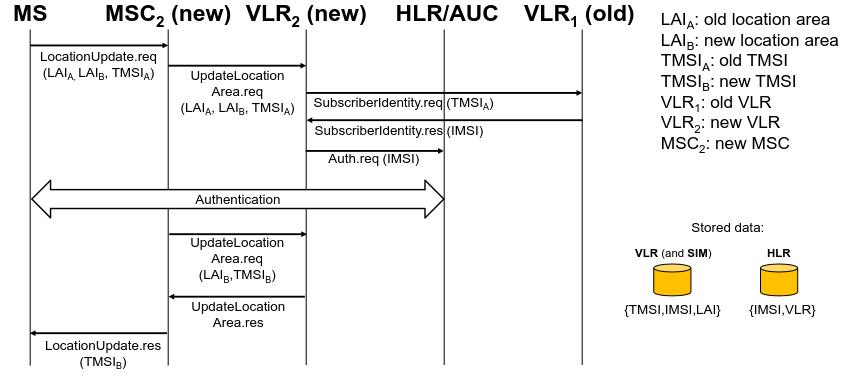
\includegraphics[width=0.8\textwidth]{pictures/9/differentMSCsequence.png}
	\end{figure}
	\begin{figure}[H]
		\centering
		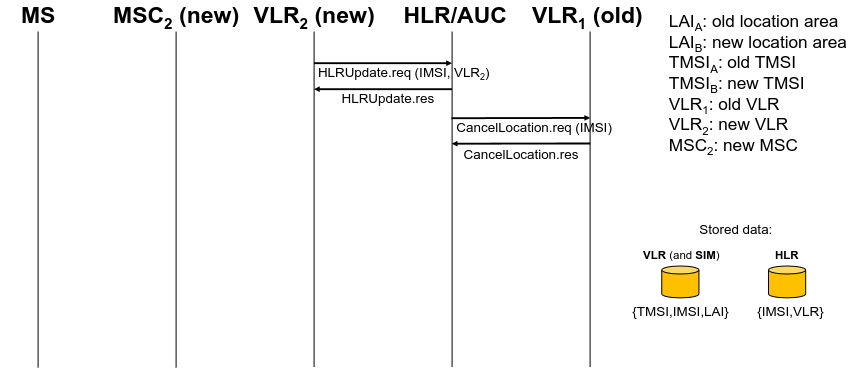
\includegraphics[width=0.8\textwidth]{pictures/9/differentMSCsequence2.png}
		\caption{Diagramma di sequenza per location update tra due LA servite da MSC/VLR diversi}
	\end{figure}
\end{itemize}
\section{Setup delle chiamate}
Dividiamo tra i casi in cui il chiamante è la MS e quando è il chiamato.
\subsection{Chiamata iniziata dalla MS}
Il processo di signaling è molto simile a quello adottato in PSTN.
La prima parte dei messaggi di signaling vengono portati su SDCCH, ma dopo le procedure di sicurezza un FACCH viene assegnato e usato.
Vengono utilizzati i messaggi standard di signaling di SS7, la procedura viene gestita dal MSC che interagisce con il BSC per allocare un canale di controllo.
\begin{figure}[H]
	\centering
	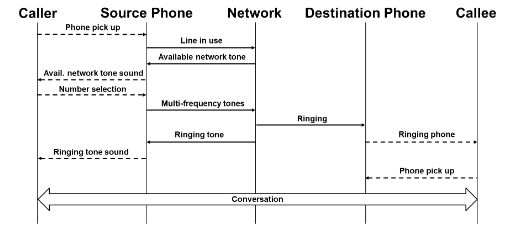
\includegraphics[width=0.8\textwidth]{pictures/9/MScalling.png}
	\caption{Chiamata iniziata dalla MS}
\end{figure}
\subsection{Chiamata ricevuta dalla MS}
Consideriamo il caso più generale, ovvero quella di una chiamata da una PSTN a una MS su una rete specifica.
Dividiamo in fasi:
\begin{enumerate}
	\item L'utente PSTN digita il MSISDN del chiamato.
	\item La rete PSTN analizza il numero e instrada la chiamata al GMSC della rete mobile del chiamato. IL GMSC è identificato dal National Destination Code (NDC) del MSISDN.
	\begin{figure}[H]
		\centering
		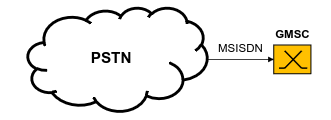
\includegraphics[width=0.5\textwidth]{pictures/9/called1.png}
	\end{figure}
	\item Il GMSC riceve la richiesta di setup della chiamata tramite signaling SS7.
	\item Il GMSC interroga l'HLR per ottenere la posizione della MS.
	\begin{figure}[H]
		\centering
		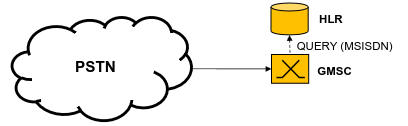
\includegraphics[width=0.6\textwidth]{pictures/9/called2.png}
	\end{figure}
	\item Il HLR analizza la query e identifica nei suoi record il VLR attualmente visitato dalla MS.
	\item Il HLR manda una routing information request al VLR includendo l'IMSI della MS.
	\item Il VLR alloca temporaneamente un MSRN per la chiamata.
	\item Il MSRN viene inoltrato al GMSC.
	\begin{figure}[H]
		\centering
		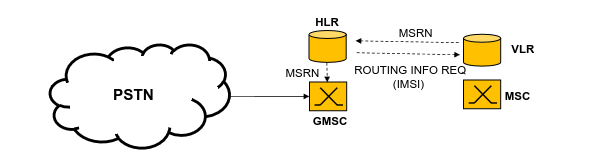
\includegraphics[width=0.8\textwidth]{pictures/9/called3.png}
	\end{figure}
	\item Il GMSC instrada la chiamata al MSC usando MSRN (signaling SS7).
	\begin{figure}[H]
		\centering
		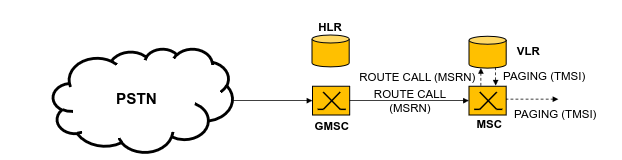
\includegraphics[width=0.8\textwidth]{pictures/9/called4.png}
	\end{figure}
	\item Il MSC attiva la procedura di paging usando il TMSI ottenuto dal VLR. In questo modo identifica la LA attualmente visitata dalla MS (il LAI è memorizzato nel VLR assieme al TMSI).
	Allora, manda un comando di paging (includendo il TMSI della MS) al BSC associato alla LA.
	\item Il BSC inoltra il messaggio di paging a tutte le BTS a cui è connesso, le quali mandando il messaggio in broadcast usando il PCH.
	\item La MS risponde al messaggio di paging e inizia una procedura di accesso (RACH/AGCH) e ottiene un SDCCH.
	\item LA MS inizia l'autenticazione e la procedura di cifratura per l'assegnamento di un TCH, in modo che si possa stabilire la chiamata.
\end{enumerate}
\subsection{Chiamata ricevuta da MS in roaming}
Ora possiamo analizzare il caso in cui la chiamata preveda il roaming.
% rivedere lezione per capire significato diagrammi
\begin{figure}[H]
	\centering
	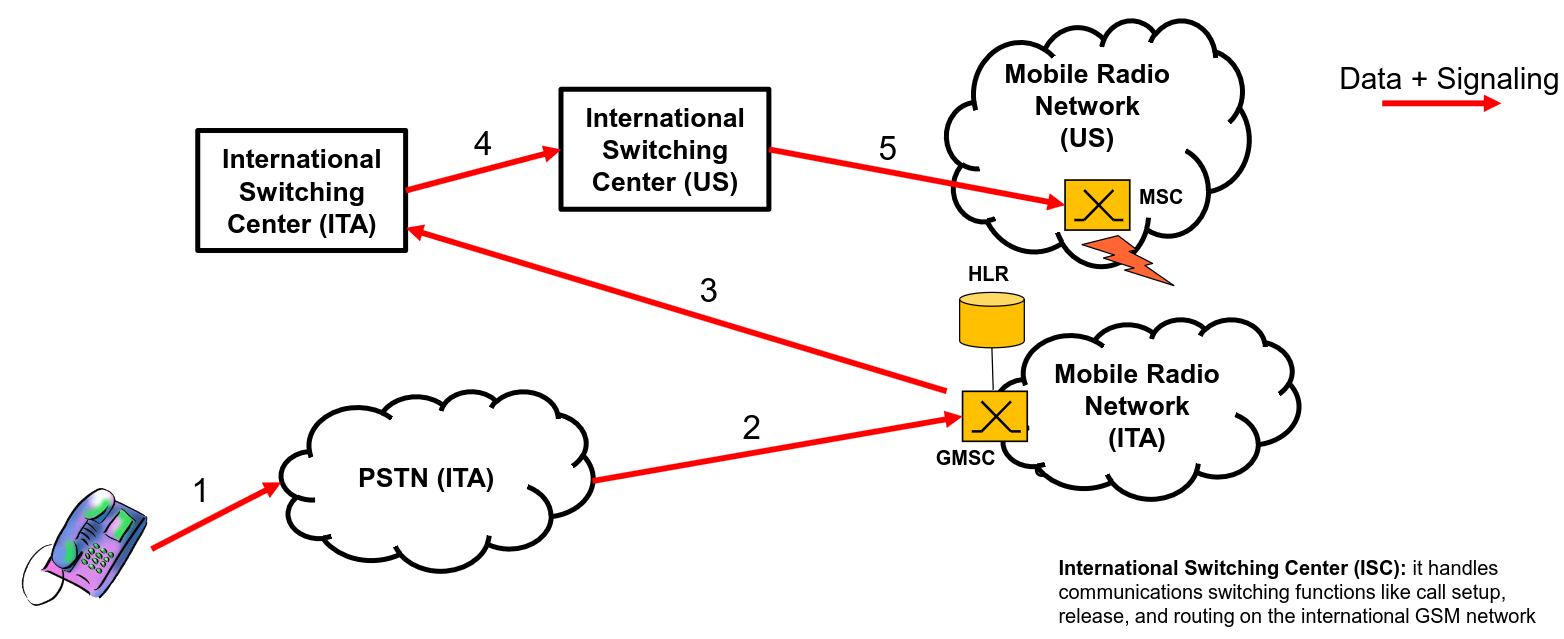
\includegraphics[width=\textwidth]{pictures/9/roaming1.png}
	\caption{Caso 1}
\end{figure}\noindent
Nel caso 1 l'utente italiano si trova in roaming negli Stati Uniti.
\begin{figure}[H]
	\centering
	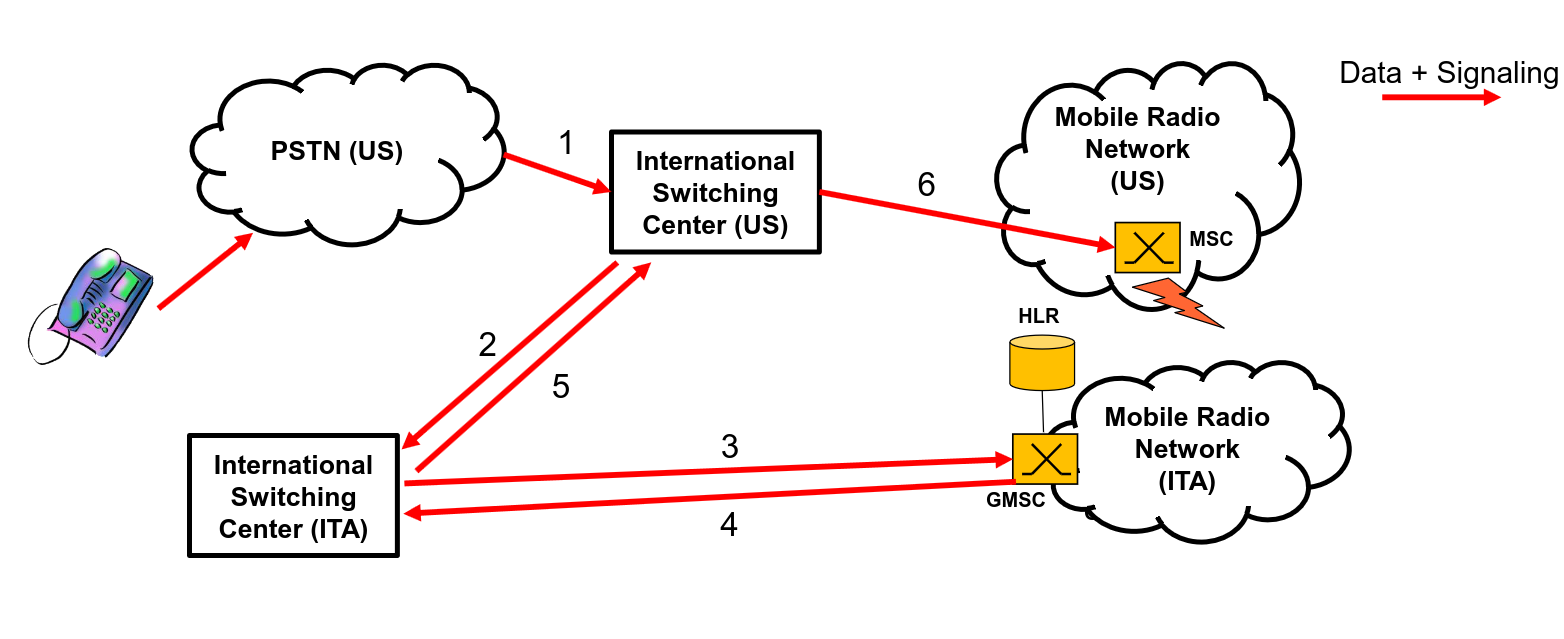
\includegraphics[width=\textwidth]{pictures/9/roaming2.png}
	\caption{Caso 2}
\end{figure}\noindent
Nel caso 2 l'utente americano vuole chiamare un utente italiano che si trova in roaming negli Stati Uniti. Notare che fino al punto 3 si assume che il chiamato sia in Italia, e quindi il GMSC della rete italiana viene contattato. In realtà, il GMSC della rete italiana non sa dove si trova l'utente, quindi interroga l'HLR per ottenere la posizione attuale. L'HLR risponde con il VLR attualmente visitato dalla MS, che si trova negli Stati Uniti. Allora il GMSC italiano inoltra la chiamata al MSC americano. N.B. in questa comunicazione vengono trasmessi sia dati che signaling, instaurando un circuito, questo è molto inefficiente. In questo caso l'utente americano paga la chiamata internazionale, sia per il flusso di dati che per il signaling!

\subsection{Mobile number portability}
% aggiungere spiegazione dalla videolezione
\begin{figure}[H]
	\centering
	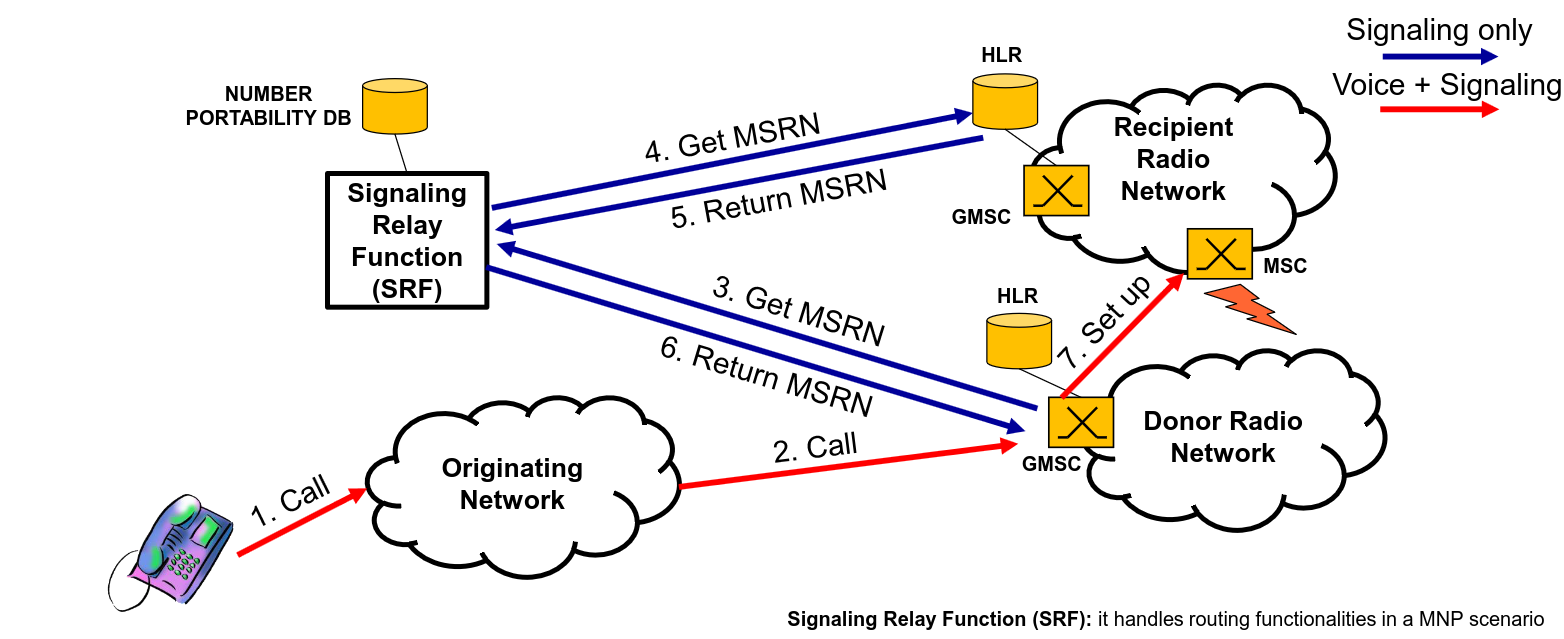
\includegraphics[width=\textwidth]{pictures/9/roaming3.png}
	\caption{Mobile number portability}
\end{figure}\noindent
Si è cercato di risolvere il problema della inefficienza di trasportare sia i dati che il signaling sulla stessa strada, introducendo il Mobile Number Portability. Naturalmente, noi sappiamo che è possibile cambiare operatore mantenendo lo stesso numero di telefono, questo è possibile distinguendo tra Donor Radio Network e Recipient Radio Network. Il Donor Radio Network è la rete originale a cui apparteneva l'utente, mentre la Recipient Radio Network è la rete a cui l'utente si è spostato. Quando il GMSC della donor riceve una chiamata per l'utente, il GMSC interroga il number portability DB con un messaggio di Get MSRN, questo viene inoltrato al GMSC della recipient che risponde. Queste interrogazioni avvengono su un flusso di solo signaling.
Dopodiché il GMSC della donor riceve la risposta, instaura il circuito tra chiamante e MSC della recipient, in cui verranno trasportati solo i dati.
\section{Handover}
La procedura viene iniziata dalla rete, ma è basata su misurazioni effettuate dalla MS (network-initiated mobile-assisted handover).
Nella mobilità attiva, l'MS scansiona i canali di controllo per ottenere informazioni sulla potenza del segnale da vari BTS, dopodiché le invia tramite SACCH.
Il BSC analizza queste misure e se necessario inizia la procedura di handover.
Ci sono tre tipi di handover:
\begin{itemize}
	\item \textbf{Intra-BSC handover}: tra due BTS collegate allo stesso BSC.
	\item \textbf{Inter-BSC handover}: tra due BTS collegate a BSC diversi, ma allo stesso MSC.
	\item \textbf{Inter-MSC handover}: tra due BTS collegate a BSC diversi e a MSC diversi.
\end{itemize}
\begin{figure}[H]
	\centering
	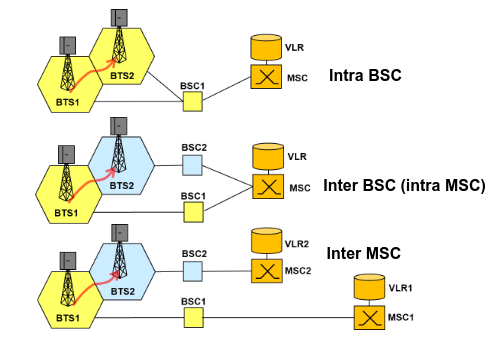
\includegraphics[width=0.5\textwidth]{pictures/9/handoverTypes.png}
	\caption{Tipi di handover in GSM}
\end{figure}
\begin{figure}[H]
	\centering
	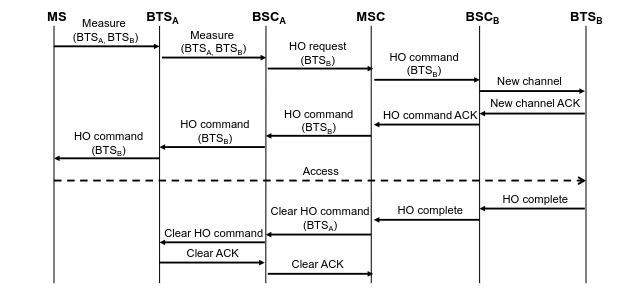
\includegraphics[width=0.8\textwidth]{pictures/9/handoverSequence.png}
	\caption{Diagramma di sequenza per handover in GSM}
\end{figure}
\section{2G-GPRS}
Il GPRS (General Packet Radio Service) è un'estensione del GSM che supporta la trasmissione di dati a pacchetto.
Vengono dedicati dei canali di traffico (PDTCH, Packet Data Traffic Channels), che vengono dinamicamente condivisi tra più MS sia per downlink che per uplink.
Inoltre vengono definiti dei nuovi canali di controllo, ad esempio per il signaling.
\textbf{EDGE} (Enhanced Data rates for GSM Evolution) è un'evoluzione del GPRS che supporta velocità di trasmissione più elevate, principalmente attraverso l'adozione di tecniche al livello fisico più efficienti.
\begin{figure}[H]
	\centering
	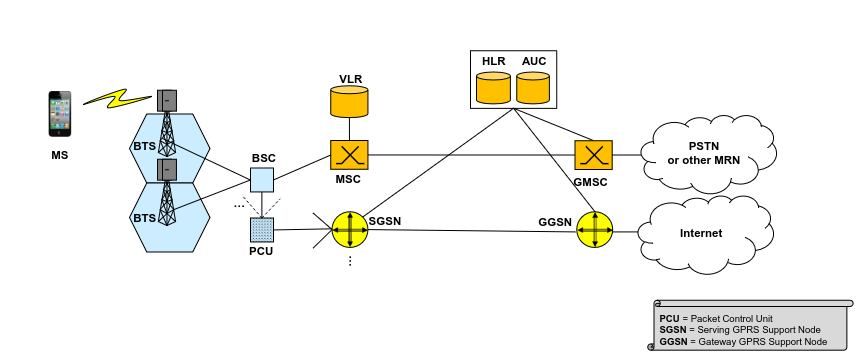
\includegraphics[width=\textwidth]{pictures/9/edge.png}
	\caption{Architettura di rete EDGE}
\end{figure}
Ora vediamo i componenti principali dell'architettura GPRS/EDGE:
\begin{itemize}
	\item \textbf{Packet Control Unit (PCU)}: equivalente a commutazione di pacchetto del BSC, gestisce le risorse radio per i canali di traffico dati.
	\item \textbf{Serving GPRS Support Node (SGSN)}: router IP che gestisce i pacchetti dati nella rete, responsabile inoltre per il controllo della mobilità e l'autenticazione.
	\item \textbf{Gateway GPRS Support Node (GGSN)}: router IP che funge da gateway tra la rete GPRS e l'Internet.
\end{itemize}
\subsection{Packet forwarding}
Il forwarding dei pacchetti IP è basato sui \textbf{tunnel}, che verranno inoltre ereditati nelle future generazioni di reti mobili.
In GPRS/EDGE ci sono due tipi di tunnel:
\begin{itemize}
	\item Un tunnel al livello due tra MS e SGSN (Logical Link Control, LLC).
	\item Un tunnel al livello 4 tra SGSN e GGSN (GPRS Tunneling Protocol, GTP).
\end{itemize}
Questo scema viene mantenuto in 3G.
\begin{figure}[H]
	\centering
	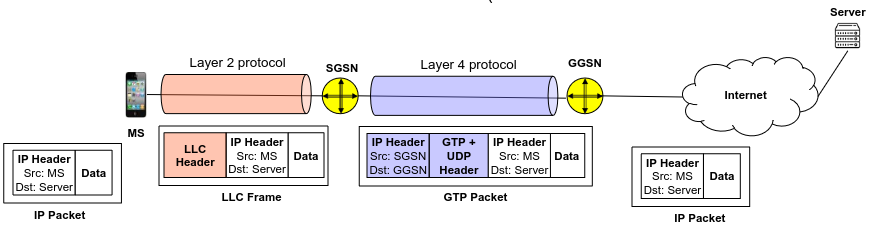
\includegraphics[width=\textwidth]{pictures/9/tunnel.png}
	\caption{Tunneling in GPRS/EDGE}
\end{figure}
I tunnel vengono usati per modificare il forwarding dei pacchetti in base alla mobilità della MS, quando è in stato attivo.
\begin{figure}[H]
	\centering
	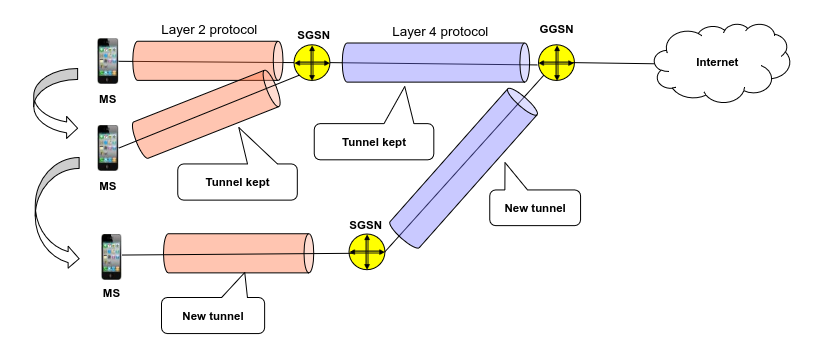
\includegraphics[width=\textwidth]{pictures/9/tunnelMobility.png}
	\caption{Tunneling e mobilità in GPRS/EDGE}
\end{figure}